\documentclass{beamer}
\usepackage{amsmath}
\usepackage[english]{babel} %set language; note: after changing this, you need to delete all auxiliary files to recompile
\usepackage[utf8]{inputenc} %define file encoding; latin1 is the other often used option
\usepackage{csquotes} % provides context sensitive quotation facilities
\usepackage{graphicx} %allows for inserting figures
\usepackage{booktabs} % for table formatting without vertical lines
\usepackage{textcomp} % allow for example using the Euro sign with \texteuro
\usepackage{stackengine}
\usepackage{wasysym}
\usepackage{tikzsymbols}
\usepackage{textcomp}
\usepackage{xcolor}
\usepackage[dvipsnames]{xcolor}

% ELIMINAR COMANDOS DE NAVEGACION%%%%%%%%%%%
\setbeamertemplate{navigation symbols}

%\newcommand{\bubblethis}[2]{
 %       \tikz[remember picture,baseline]{\node[anchor=base,inner sep=0,outer sep=0]%
 %       (#1) {\underline{#1}};\node[overlay,cloud callout,callout relative pointer={(0.2cm,-0.7cm)},%
 %       aspect=2.5,fill=yellow!90] at ($(#1.north)+(-0.5cm,1.6cm)$) {#2};}%
 %   }%
%\tikzset{face/.style={shape=circle,minimum size=4ex,shading=radial,outer sep=0pt,
 %       inner color=white!50!yellow,outer color= yellow!70!orange}}

%% Some commands to make the code easier
\newcommand{\emoticon}[1][]{%
  \node[face,#1] (emoticon) {};
  %% The eyes are fixed.
  \draw[fill=white] (-1ex,0ex) ..controls (-0.5ex,0.2ex)and(0.5ex,0.2ex)..
        (1ex,0.0ex) ..controls ( 1.5ex,1.5ex)and( 0.2ex,1.7ex)..
        (0ex,0.4ex) ..controls (-0.2ex,1.7ex)and(-1.5ex,1.5ex)..
        (-1ex,0ex)--cycle;}
\newcommand{\pupils}{
  %% standard pupils
  \fill[shift={(0.5ex,0.5ex)},rotate=80] 
       (0,0) ellipse (0.3ex and 0.15ex);
  \fill[shift={(-0.5ex,0.5ex)},rotate=100] 
       (0,0) ellipse (0.3ex and 0.15ex);}

\newcommand{\emoticonname}[1]{
  \node[below=1ex of emoticon,font=\footnotesize,
        minimum width=4cm]{#1};}
\usepackage{scalerel}
\usetikzlibrary{positioning}
\usepackage{xcolor,amssymb}
\newcommand\dangersignb[1][2ex]{%
  \scaleto{\stackengine{0.3pt}{\scalebox{1.1}[.9]{%
  \color{red}$\blacktriangle$}}{\tiny\bfseries !}{O}{c}{F}{F}{L}}{#1}%
}
\newcommand\dangersignw[1][2ex]{%
  \scaleto{\stackengine{0.3pt}{\scalebox{1.1}[.9]{%
  \color{red}$\blacktriangle$}}{\color{white}\tiny\bfseries !}{O}{c}{F}{F}{L}}{#1}%
}
\usepackage{fontawesome} % Social Icons
\usepackage{epstopdf} % allow embedding eps-figures
\usepackage{tikz} % allows drawing figures
\usepackage{amsmath,amssymb,amsthm} %advanced math facilities
\usepackage{lmodern} %uses font that support italic and bold at the same time
\usepackage{hyperref}
\usepackage{tikz}
\hypersetup{
    colorlinks=true,
    linkcolor=blue,
    filecolor=magenta,      
    urlcolor=blue,
}
\usepackage{tcolorbox}
%add citation management using BibLaTeX
\usepackage[citestyle=authoryear-comp, %define style for citations
    bibstyle=authoryear-comp, %define style for bibliography
    maxbibnames=10, %maximum number of authors displayed in bibliography
    minbibnames=1, %minimum number of authors displayed in bibliography
    maxcitenames=3, %maximum number of authors displayed in citations before using et al.
    minnames=1, %maximum number of authors displayed in citations before using et al.
    datezeros=false, % do not print dates with leading zeros
    date=long, %use long formats for dates
    isbn=false,% show no ISBNs in bibliography (applies only if not a mandatory field)
    url=false,% show no urls in bibliography (applies only if not a mandatory field)
    doi=false, % show no dois in bibliography (applies only if not a mandatory field)
    eprint=false, %show no eprint-field in bibliography (applies only if not a mandatory field)
    backend=biber %use biber as the backend; backend=bibtex is less powerful, but easier to install
    ]{biblatex}
\addbibresource{../mybibfile.bib} %define bib-file located one folder higher


\usefonttheme[onlymath]{serif} %set math font to serif ones

\definecolor{beamerblue}{rgb}{0.2,0.2,0.7} %define beamerblue color for later use

%%% defines highlight command to set text blue
\newcommand{\highlight}[1]{{\color{blue}{#1}}}


%%%%%%% commands defining backup slides so that frame numbering is correct

\newcommand{\backupbegin}{
   \newcounter{framenumberappendix}
   \setcounter{framenumberappendix}{\value{framenumber}}
}
\newcommand{\backupend}{
   \addtocounter{framenumberappendix}{-\value{framenumber}}
   \addtocounter{framenumber}{\value{framenumberappendix}}
}

%%%% end of defining backup slides

%Specify figure caption, see also http://tex.stackexchange.com/questions/155738/caption-package-not-working-with-beamer
\setbeamertemplate{caption}{\insertcaption} %redefines caption to remove label "Figure".
%\setbeamerfont{caption}{size=\scriptsize,shape=\itshape,series=\bfseries} %sets figure  caption bold and italic and makes it smaller


\usetheme{Boadilla}

%set options of hyperref package
\hypersetup{
    bookmarksnumbered=true, %put section numbers in bookmarks
    naturalnames=true, %use LATEX-computed names for links
    citebordercolor={1 1 1}, %color of border around cites, here: white, i.e. invisible
    linkbordercolor={1 1 1}, %color of border around links, here: white, i.e. invisible
    colorlinks=true, %color links
    anchorcolor=black, %set color of anchors
    linkcolor=beamerblue, %set link color to beamer blue
    citecolor=blue, %set cite color to beamer blue
    pdfpagemode=UseThumbs, %set default mode of PDF display
    breaklinks=true, %break long links
    pdfstartpage=1 %start at first page
    }

\newtcolorbox{boxA}{
    fontupper = \bf,
    boxrule = 1.5pt,
    colframe = black % frame color
}
\newtcolorbox{boxB}{
    boxrule = 1.5pt,
    colframe = blue!70!black,, % frame color
    colback = blue!7!white,
}

% --------------------
% Overall information
% --------------------
\title[Economía I]{Economía I \vspace{4mm}
\\ Magistral 4}
\date{}
\author[Victoria Rosino]{Victoria Rosino}
\vspace{0.4cm}
\institute[]{Universidad de San Andrés} 

\begin{document}

\begin{frame}
\vspace{0.4cm}
\titlepage
\centering
\vspace{-0.7cm}

\includegraphics[scale=0.3]{Slides Principios de Economia/Figures/udesa_logo.jpg} 
\end{frame}


\begin{frame}
\frametitle{Retomemos}
\begin{itemize}
  \item Hasta ahora, hemos visto cómo un individuo toma decisiones de consumo
  \item Dada su restricción presupuestaria, elegía la canasta de consumo que se situaba en la curva de indiferencia más lejana del origen
  \item Luego vimos qué sucedía cuando cambiaba el nivel de ingreso y cuando se movía en precio de uno de los bienes (efecto ingreso y efecto sustitución) 
  \item Hoy veremos cómo esto se traslada a una curva de demanda individual.
\end{itemize}
\end{frame}

\begin{frame}
\frametitle{Así terminamos}
\begin{center}
\begin{figure}[H]
\renewcommand{\figurename}{Figure}
\begin{center}
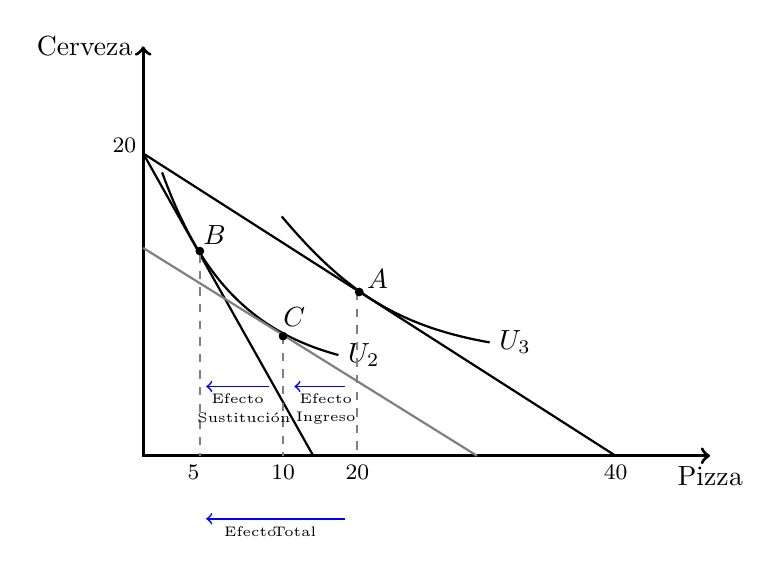
\begin{tikzpicture}[scale=0.8]
\draw[very thick,<->] (0,6.5) node[left]{Cerveza}--(0,0)--(9,0) node[below]{Pizza};
\draw [thick] (2.2,3.8) to [out=310,in=170] (5.5,1.8);
\node [right] at (5.5,1.8) {$U_3$};
\draw [thick] (0.3,4.5) to [out=290,in=165] (3.1,1.6);
\node [right] at (3.1,1.6) {$U_2$};
\node[below] at (3.4,0) {\footnotesize 20};
\node[below] at (7.5,0) {\footnotesize 40};
\node[below] at (-0.3,5.2) {\footnotesize 20};
\node[below] at (2.22,0) {\footnotesize 10};
\node[below] at (0.8,0) {\footnotesize 5};
\draw [thick] (0,4.8) -- (7.5,0);
\draw [thick] (0,4.8) -- (2.7,0);
\draw[thick, dashed,gray](0.9,3.2)--(0.9,0);
\draw[thick, dashed,gray](3.4,2.6)--(3.4,0);
\draw[thick, dashed,gray](2.22,1.9)--(2.22,0);
\draw [thick, gray] (0,3.3) -- (5.3,0);
\draw[semithick, blue, <-] (1,-1)--(3.2,-1);
\node[] at (1.7,-1.2){\tiny Efecto};
\node[] at (2.4,-1.2){\tiny Total};
\draw[semithick, blue, <-] (2.4,1.1)--(3.2,1.1);
\node[] at (2.9,0.9){\tiny Efecto};
\node[] at (2.9,0.6){\tiny Ingreso};
\draw[semithick, blue, <-] (1,1.1)--(2,1.1);
\node[] at (1.5,0.9){\tiny Efecto};
\node[] at (1.6,0.6){\tiny Sustitución};
\node [above] at (2.4,1.9) {$C$};
\draw[fill] (2.22,1.9) circle [radius =0.06];
\node [right] at (0.8,3.5) {$B$};
\draw[fill] (0.9,3.25) circle [radius =0.06];
\node [right] at (3.4,2.8) {$A$};
\draw[fill] (3.43,2.6) circle [radius =0.06];
\end{tikzpicture}
\end{center}
\end{figure}
\end{center}
\end{frame}


\begin{frame}
\frametitle{Cambios en el precio de la pizza}
\begin{itemize}
    \item Si mantenemos constantes el ingreso del individuo y el precio de la cerveza, ¿cómo afectará un cambio en el precio de la pizza a la cantidad de pizza que adquiera el consumidor? \vspace{2mm}
    \begin{itemize}
         \item La canasta de bienes óptima es la que resulta de igualar la pendiente de la curva de indiferencia con la pendiente de la restricción presupuestaria. 
    \end{itemize}
\end{itemize}
\end{frame}

\begin{frame}
\frametitle{Si aumenta el precio de la pizza:}
\begin{center}
\begin{figure}[H]
\renewcommand{\figurename}{Figure}
\begin{center}
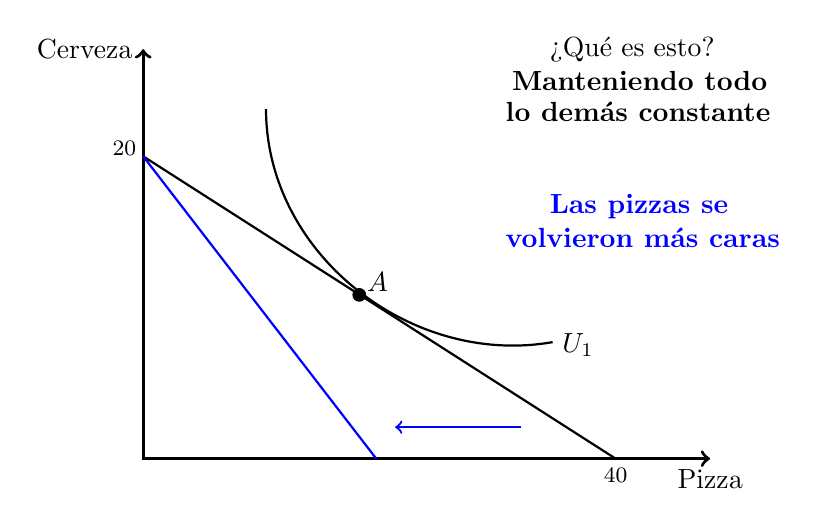
\begin{tikzpicture}[scale=0.8]
\draw[very thick,<->] (0,6.5) node[left]{Cerveza}--(0,0)--(9,0) node[below]{Pizza};
\draw [thick] (1.95,5.55) to [out=270,in=190] (6.5,1.85);
\node [right] at (6.5,1.8) {$U_1$};
\node[below] at (7.5,0) {\footnotesize 40};
\draw [thick] (0,4.8) -- (7.5,0);
\draw [thick, blue] (0,4.8) -- (3.7,0);
\node[below] at (-0.3,5.2) {\footnotesize 20};
\node [right] at (3.4,2.8) {$A$};
\draw[fill] (3.43,2.6) circle [radius =0.1];
\node[right] at (6.3,6.5) {¿Qué es esto?};
\node[right] at (5.7,6) {\textbf{Manteniendo todo}};
\node[right] at (5.6,5.5) {\textbf{lo demás constante}};
\draw[->, thick, blue] (6,0.5) -- (4,0.5);
\node[right, blue] at (6.3,4) {\textbf{Las pizzas se}};
\node[right, blue] at (5.6,3.5) {\textbf{volvieron más caras}};
\end{tikzpicture}
\end{center}
\end{figure}
\end{center}
\end{frame}


\begin{frame}
\frametitle{El nuevo equilibrio es B}
\begin{center}
\begin{figure}[H]
\renewcommand{\figurename}{Figure}
\begin{center}
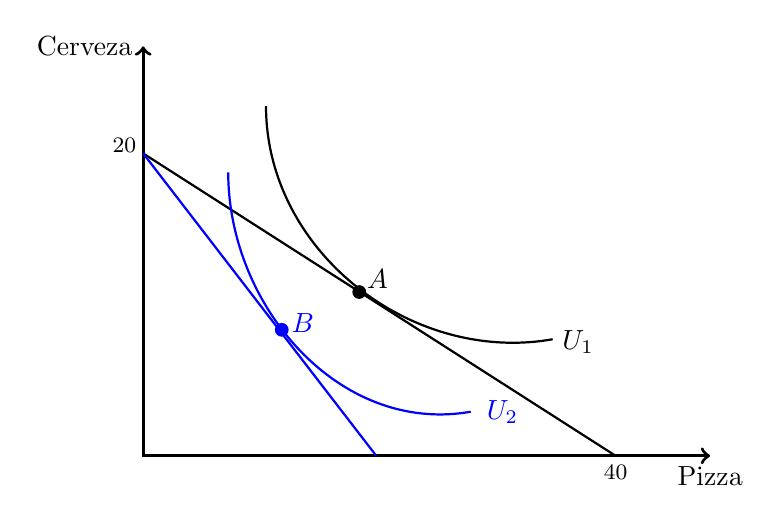
\begin{tikzpicture}[scale=0.8]
\draw[very thick,<->] (0,6.5) node[left]{Cerveza}--(0,0)--(9,0) node[below]{Pizza};
\draw [thick] (1.95,5.55) to [out=270,in=190] (6.5,1.85);
\node [right] at (6.5,1.8) {$U_1$};
\node[below] at (7.5,0) {\footnotesize 40};
\draw [thick] (0,4.8) -- (7.5,0);
\draw [thick, blue] (0,4.8) -- (3.7,0);
\node[below] at (-0.3,5.2) {\footnotesize 20};
\node [right] at (3.4,2.8) {$A$};
\draw[fill] (3.43,2.6) circle [radius =0.1];
\draw [thick, blue] (1.35,4.5) to [out=270,in=190] (5.2,0.7);
\node [right, blue] at (5.3,0.7) {$U_2$};
\node [right, blue] at (2.2,2.1) {$B$};
\draw[fill, blue] (2.2,2) circle [radius =0.1];
\end{tikzpicture}
\end{center}
\end{figure}
\end{center}
\end{frame}

\begin{frame}
\frametitle{Pensemos un minuto qué estamos haciendo...}
\begin{itemize}
    \item Cuando realizamos este ejercicio, estamos obteniendo las cantidades del bien que el individuo está dispuesto a consumir (dado su presupuesto) a cada precio... \vspace{2mm}
    \item Entonces, si repetimos el ejercicio varias veces, podríamos ver qué sucede con las cantidades demandadas del consumidor cada vez que el precio aumenta un poquito más.
\end{itemize}
\end{frame}

\begin{frame}
\frametitle{Repitamos el ejercicio de pensar qué sucede si cambian los precios... primero el precio es \$50}
\begin{center}
  \begin{minipage}{0.48\textwidth}
      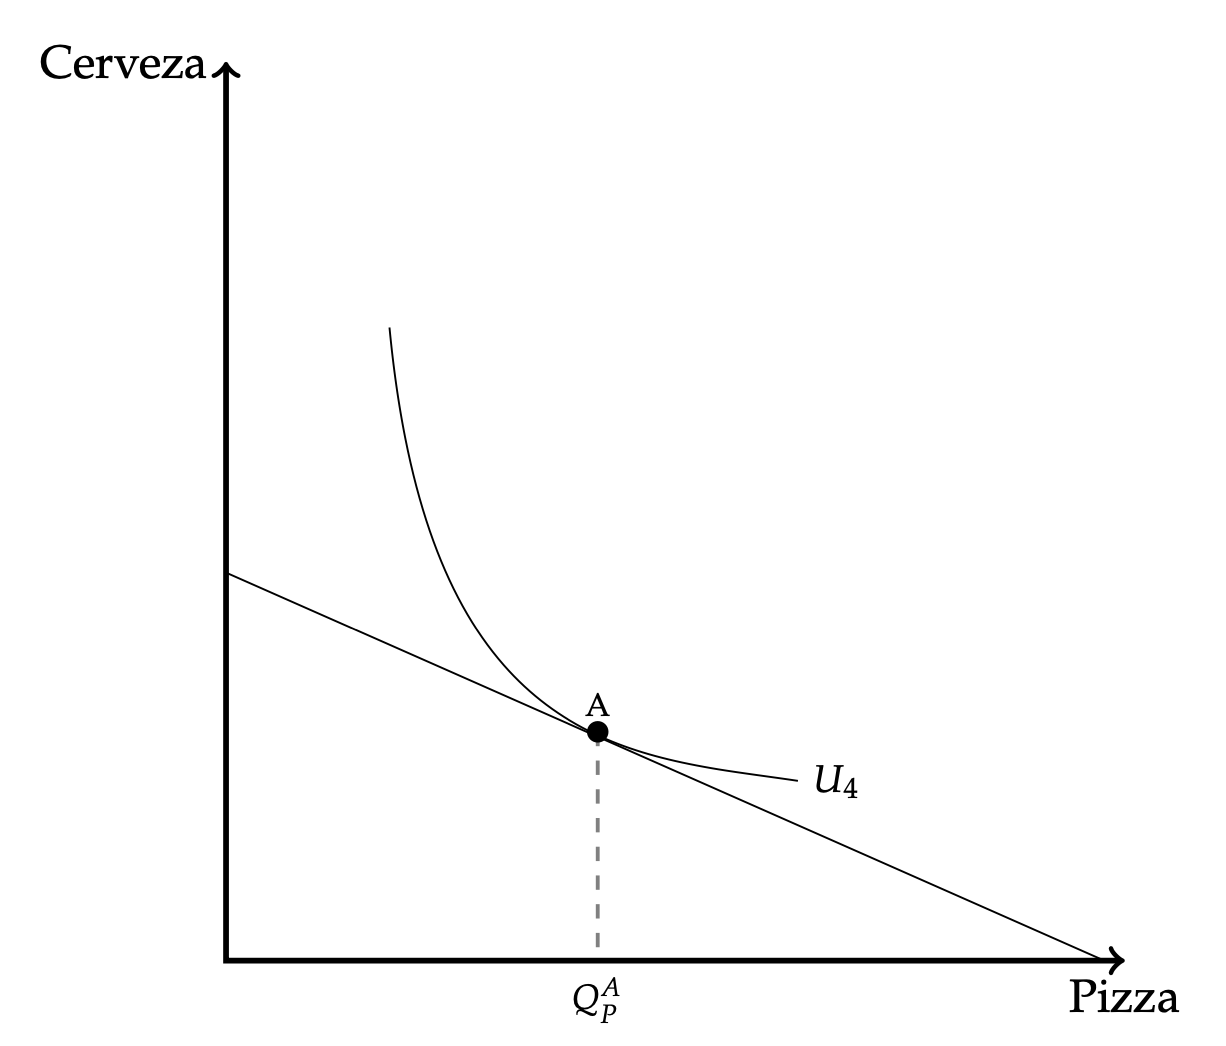
\includegraphics[width=\linewidth]{Slides Principios de Economia/Figures/Magistral_04/C8.11.png}
  \end{minipage}\hfill
  \begin{minipage}{0.48\textwidth}
      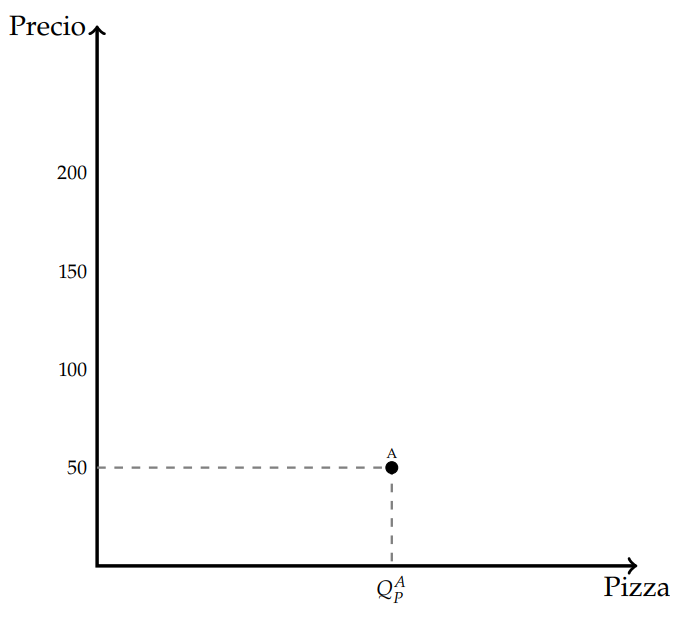
\includegraphics[width=\linewidth]{Slides Principios de Economia/Figures/Magistral_04/C8.12.png}
  \end{minipage}
\end{center}
\end{frame}

\begin{frame}
\frametitle{Ahora el precio es \$100:}
\begin{center}
  \begin{minipage}{0.48\textwidth}
      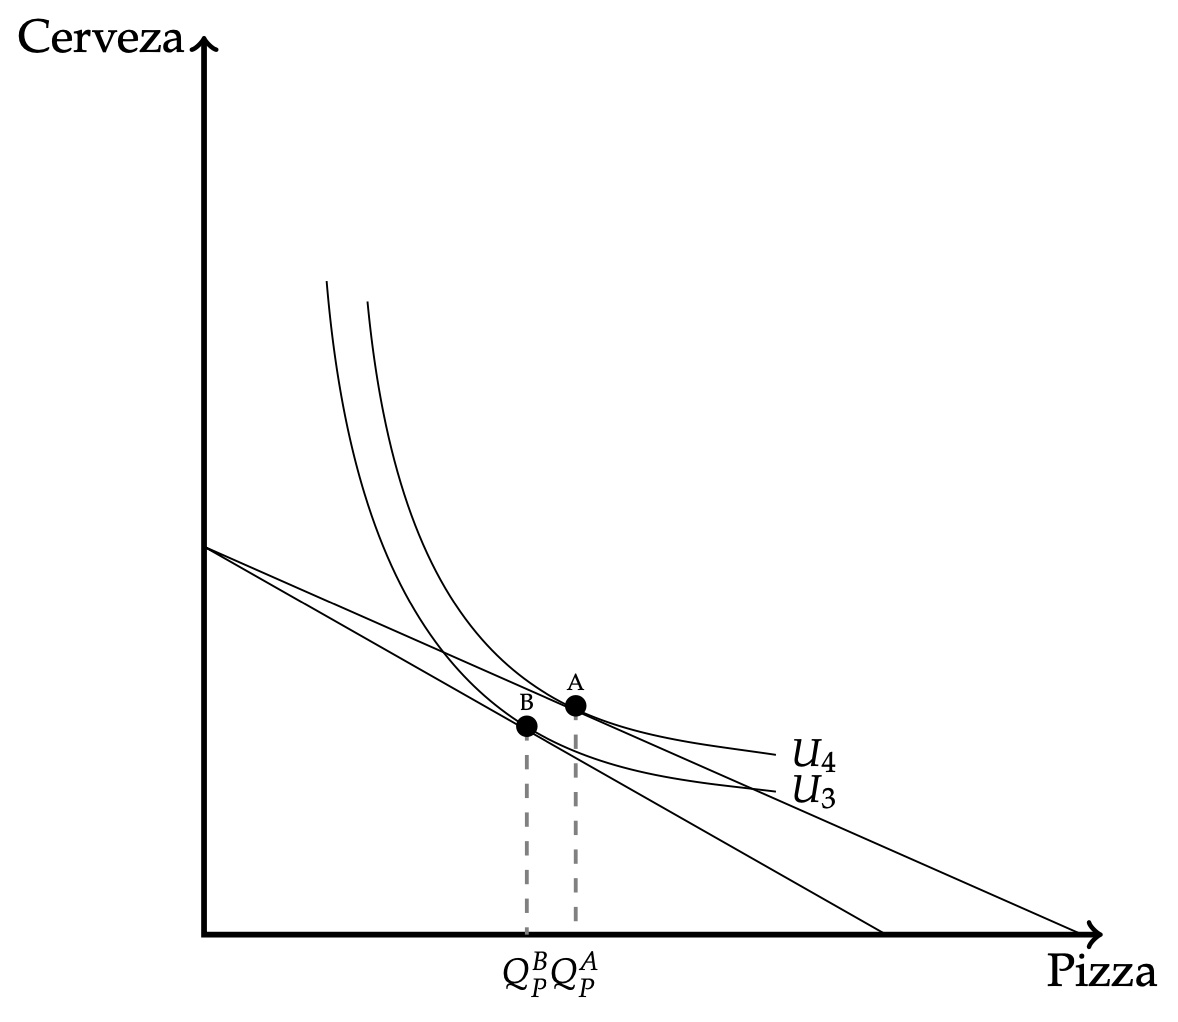
\includegraphics[width=\linewidth]{Slides Principios de Economia/Figures/Magistral_04/C8.13.png}
  \end{minipage}\hfill
  \begin{minipage}{0.48\textwidth}
      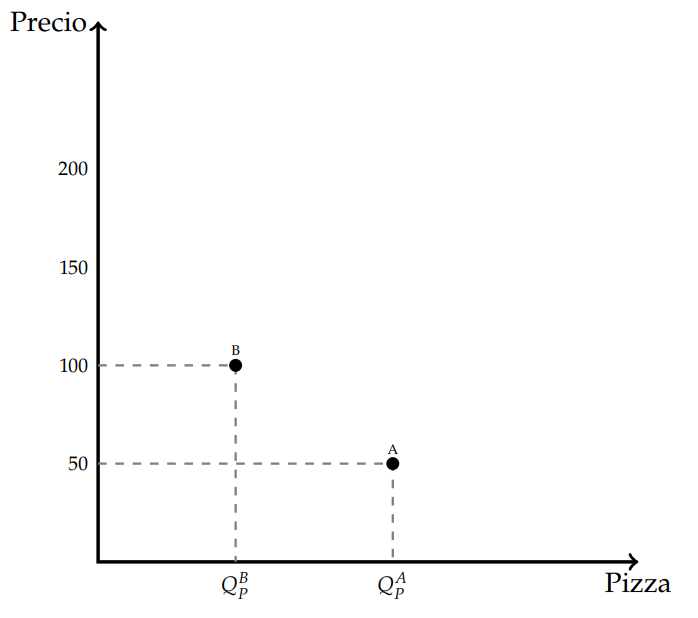
\includegraphics[width=\linewidth]{Slides Principios de Economia/Figures/Magistral_04/C8.14.png}
  \end{minipage}
\end{center}
\end{frame}


\begin{frame}
\frametitle{Y si seguimos aumentando de a \$50...}
\begin{center}
  \begin{minipage}{0.48\textwidth}
      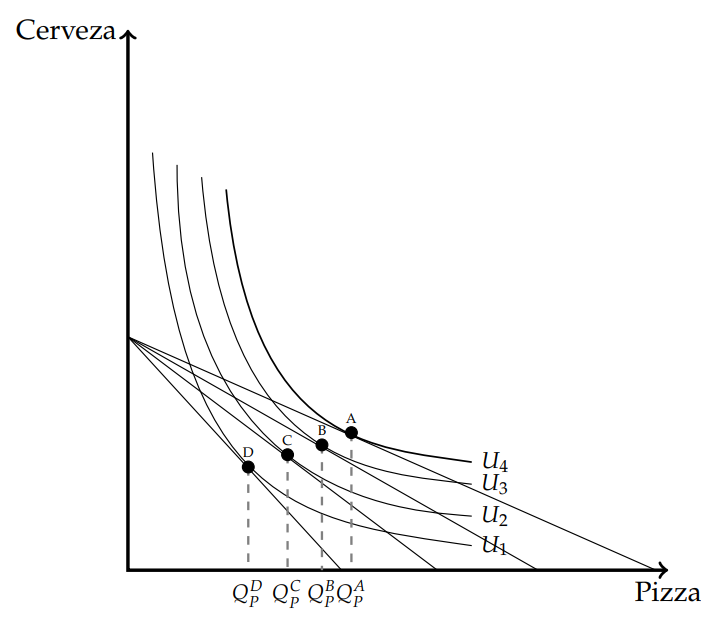
\includegraphics[width=\linewidth]{Slides Principios de Economia/Figures/Magistral_04/C8.15.png}
  \end{minipage}\hfill
  \begin{minipage}{0.48\textwidth}
      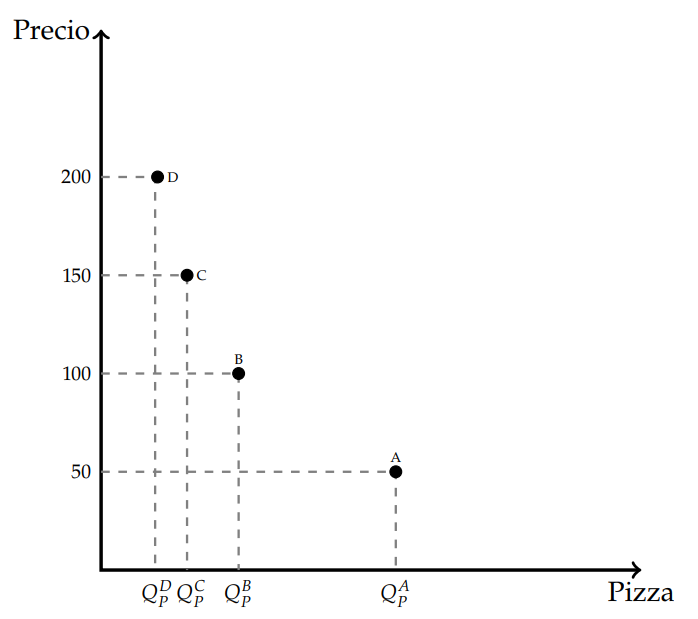
\includegraphics[width=\linewidth]{Slides Principios de Economia/Figures/Magistral_04/C8.16.png}
  \end{minipage}
\end{center}
\end{frame}

\begin{frame}
\frametitle{... obtenemos la curva de demanda del estudiante}
\begin{center}
  \begin{minipage}{0.48\textwidth}
      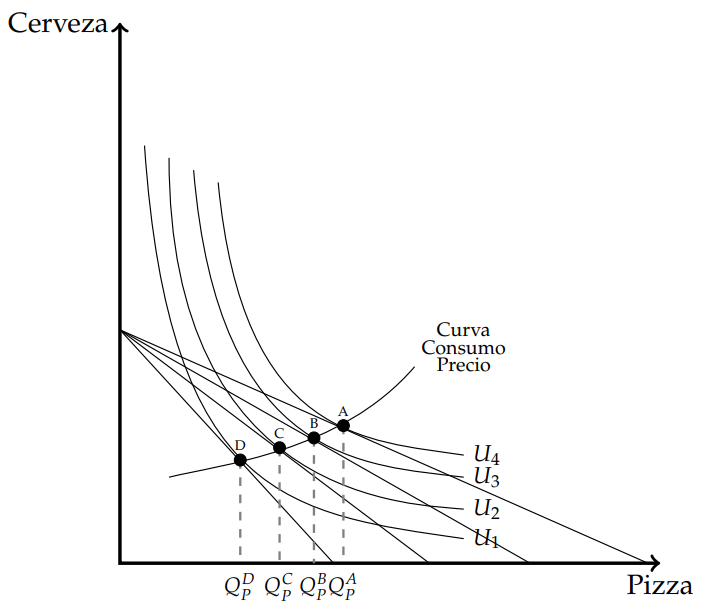
\includegraphics[width=\linewidth]{Slides Principios de Economia/Figures/Magistral_04/C8.17.png}
  \end{minipage}\hfill
  \begin{minipage}{0.48\textwidth}
      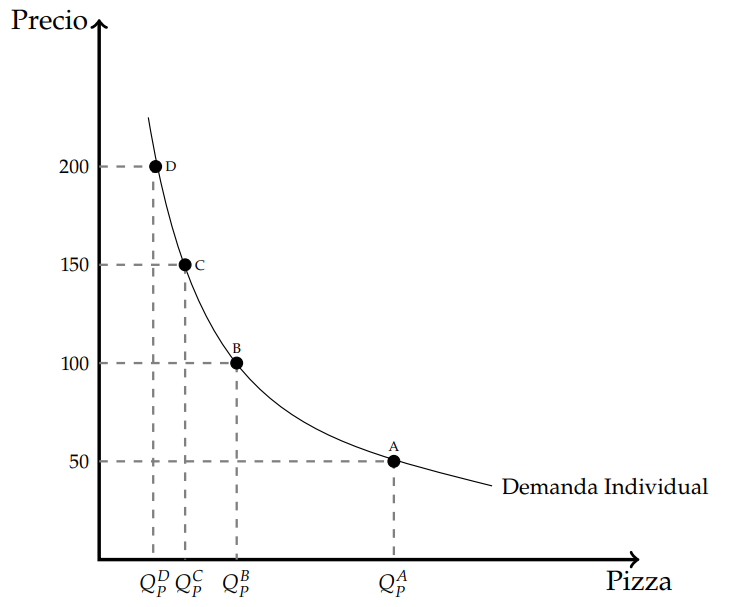
\includegraphics[width=\linewidth]{Slides Principios de Economia/Figures/Magistral_04/C8.18.png}
  \end{minipage}
\end{center}
\vspace{3mm}
El conjunto de canastas de consumo óptimas forman lo que denominamos la \textbf{curva precio-consumo}.
\end{frame}

\begin{frame}
\frametitle{La curva de demanda individual}
    \begin{boxB}
    \begin{center}
    La \textbf{demanda individual} es la cantidad de un bien que un individuo está dispuesto a comprar a cada precio.
    \end{center}
    \end{boxB}
    \begin{itemize}
    \item En nuestro ejemplo, tenemos la curva de demanda de pizza, que nos indica la cantidad de porciones de pizza que Paula está dispuesta a comprar para cada precio de la porción de pizza. \vspace{3mm}
    \item Alternativamente, podemos interpretar cada punto de la curva de demanda como la máxima disposición a pagar del consumidor, dada una cantidad de bienes.
    \end{itemize}
\end{frame}


\begin{frame}
\frametitle{¿Cómo construimos la curva de demanda del mercado?}
Supongamos que hay dos consumidores con la misma demanda individual \vspace{1mm}
\begin{figure}[H]
\begin{center}
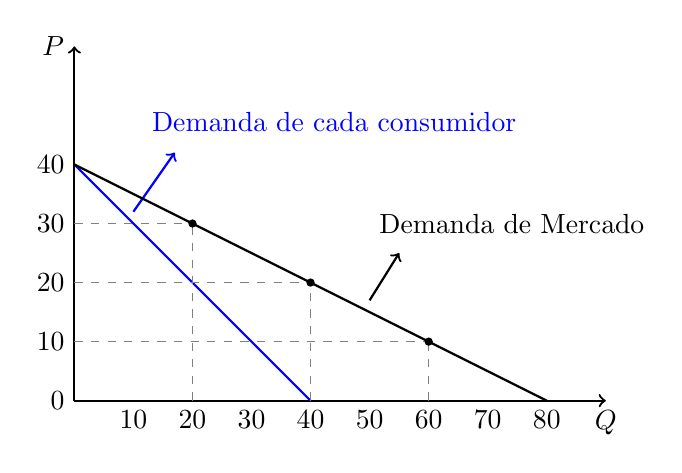
\begin{tikzpicture}[scale=0.75]
    % Configuración de ejes
    \draw[thick,->] (0,0) -- (9,0) node[below] {$Q$};
    \draw[thick,->] (0,0) -- (0,6) node[left] {$P$};
    
    % Curva de demanda individual
    \draw[thick, color=blue] (0,4) -- (4,0);
    \node[above, blue] at (4.4,4.4) {Demanda de cada consumidor};
    \draw[->, thick, blue] (1,3.2) -- (1.7,4.2);

    % Curva de demanda del mercado
    \draw[thick] (0,4) -- (8,0);
    \node[right] at (5,3) {Demanda de Mercado};
    \draw[->, thick] (5,1.7) -- (5.5,2.5);

    % Líneas punteadas
    \draw[dashed, gray] (2,0) -- (2,3);
    \draw[dashed, gray] (4,0) -- (4,2);
    \draw[dashed, gray] (6,0) -- (6,1);
    \draw[dashed, gray] (0,3) -- (2,3);
    \draw[dashed, gray] (0,2) -- (4,2);
    \draw[dashed, gray] (0,1) -- (6,1);
    
    % Etiquetas de puntos
    \fill (2,3) circle (2pt);
    \fill (4,2) circle (2pt);
    \fill (6,1) circle (2pt);
    
    % Etiquetas eje Y
    \node[left] at (0,4) {40};
    \node[left] at (0,3) {30};
    \node[left] at (0,2) {20};
    \node[left] at (0,1) {10};

    % Etiquetas eje X
    \node[below] at (1,0) {10};
    \node[below] at (2,0) {20};
    \node[below] at (3,0) {30};
    \node[below] at (4,0) {40};
    \node[below] at (5,0) {50};
    \node[below] at (6,0) {60};
    \node[below] at (7,0) {70};
    \node[below] at (8,0) {80};
    \node[left] at (0,0) {0};

\end{tikzpicture}
\end{center}
\end{figure}
\centering Para cada precio, tenemos que sumar las cantidades individuales demandadas de todos los consumidores
\end{frame}

\begin{frame}
  \frametitle{¿Y si tenemos demandas individuales distintas?}
\begin{figure}[H]
\begin{center}
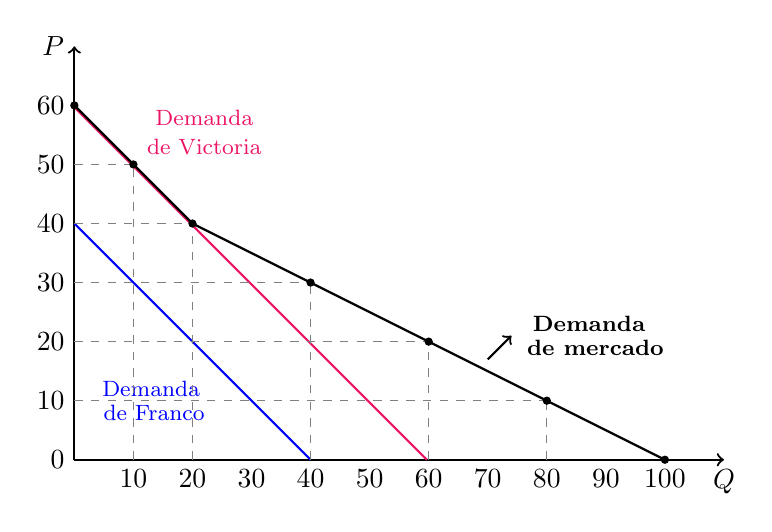
\begin{tikzpicture}[scale=0.75]
    % Configuración de ejes
    \draw[thick,->] (0,0) -- (11,0) node[below] {$Q$};
    \draw[thick,->] (0,0) -- (0,7) node[left] {$P$};
    
    % Curva de demanda Franco
    \draw[thick, color=blue] (0,4) -- (4,0);
    \node[above, blue] at (1.3,0.9) {\footnotesize Demanda};
    \node[above, blue] at (1.35,0.5) {\footnotesize de Franco};

    % Curva de demanda Victoria
    \draw[thick, color=WildStrawberry] (0,5.97) -- (5.97,0);
    \node[above, WildStrawberry] at (2.2,5.5) {\footnotesize Demanda};
    \node[above, WildStrawberry] at (2.2,5) {\footnotesize de Victoria};

    % Curva de demanda del mercado
    \draw[thick] (0,6) -- (2,4) -- (10,0);
    \node[right] at (7.6,2.3) {\footnotesize \textbf{Demanda}};
    \node[right] at (7.5,1.9) {\footnotesize \textbf{de mercado}};
    \draw[->, thick] (7,1.7) -- (7.4,2.1);

    % Líneas punteadas
    \draw[dashed, gray] (1,0) -- (1,5);
    \draw[dashed, gray] (2,0) -- (2,4);
    \draw[dashed, gray] (4,0) -- (4,3);
    \draw[dashed, gray] (6,0) -- (6,2);
    \draw[dashed, gray] (8,0) -- (8,1);
    \draw[dashed, gray] (0,5) -- (1,5);
    \draw[dashed, gray] (0,4) -- (2,4);
    \draw[dashed, gray] (0,3) -- (4,3);
    \draw[dashed, gray] (0,2) -- (6,2);
    \draw[dashed, gray] (0,1) -- (8,1);
    
    % Etiquetas de puntos
    \fill (0,6) circle (2pt);
    \fill (1,5) circle (2pt);
    \fill (2,4) circle (2pt);
    \fill (4,3) circle (2pt);
    \fill (6,2) circle (2pt);
    \fill (8,1) circle (2pt);
    \fill (10,0) circle (2pt);
    
    % Etiquetas eje Y
    \node[left] at (0,6) {60};
    \node[left] at (0,5) {50};
    \node[left] at (0,4) {40};
    \node[left] at (0,3) {30};
    \node[left] at (0,2) {20};
    \node[left] at (0,1) {10};

    % Etiquetas eje X
    \node[below] at (1,0) {10};
    \node[below] at (2,0) {20};
    \node[below] at (3,0) {30};
    \node[below] at (4,0) {40};
    \node[below] at (5,0) {50};
    \node[below] at (6,0) {60};
    \node[below] at (7,0) {70};
    \node[below] at (8,0) {80};
    \node[below] at (9,0) {90};
    \node[below] at (10,0) {100};

    \node[left] at (0,0) {0};

\end{tikzpicture}
\end{center}
\end{figure}
Seguimos sumando las cantidades demandadas a cada precio. Pero pueden haber puntos en donde solo demanda una sola persona, como en $P = 50$

\end{frame}

\begin{frame}
\frametitle{¿Qué es la demanda?}
    \begin{itemize}
        \item La curva de demanda muestra cuál es la cantidad máxima del bien que están dispuestos a consumir los individuos a \textit{cada precio}, o \vspace{2mm}
        \item ...  cuál es la disposición máxima a pagar de los consumidores para \textit{cada cantidad} del bien.
    \end{itemize}
    \begin{center}
    \begin{figure}[H]
    \renewcommand{\figurename}{Figure}
    \begin{center}
        \begin{tikzpicture}[scale=0.65]
        \draw[thick,->] (0,0) -- (7,0) node[below] {$Q$};
        \draw[thick,->] (0,0) -- (0,6.5) node[left] {$P$};
        \draw [thick] (1,5.5) -- (6,1);
        \node [right] at (6,1) {$D$};
        \node [right] at (3.2,3.7) {$A$};
        \fill (3.2,3.5) circle (3pt);
        \draw[dashed, gray] (3.2,0) -- (3.2,3.5);
        \draw[dashed, gray] (0,3.5) -- (3.2,3.5);
        \node[below] at (3.2,0) {40};
        \node[left] at (0,3.5) {30};
        \end{tikzpicture}
    \end{center}
    \end{figure}
    \end{center}
\end{frame}



\begin{frame}
\frametitle{Desplazamientos \textbf{sobre} la curva de demanda}

    \begin{itemize}
        \item Si cambia el \textbf{precio} de un bien, se modifica su \textbf{cantidad demandada}.\vspace{2mm}
        \item La curva de demanda no se modifica, nos desplazamos \textbf{sobre} la curva.\vspace{2mm}
    \end{itemize}
    \begin{center}
    \begin{figure}[H]
    \renewcommand{\figurename}{Figure}
    \begin{center}
        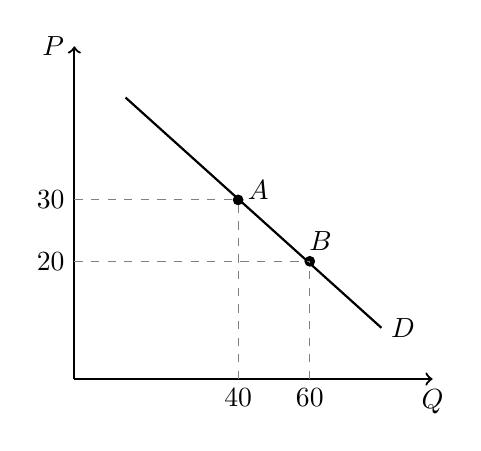
\begin{tikzpicture}[scale=0.65]
        \draw[thick,->] (0,0) -- (7,0) node[below] {$Q$};
        \draw[thick,->] (0,0) -- (0,6.5) node[left] {$P$};
        \draw [thick] (1,5.5) -- (6,1);
        \node [right] at (6,1) {$D$};

        % Punto A
        \node [right] at (3.2,3.7) {$A$};
        \fill (3.2,3.5) circle (3pt);
        \draw[dashed, gray] (3.2,0) -- (3.2,3.5);
        \draw[dashed, gray] (0,3.5) -- (3.2,3.5);
        \node[below] at (3.2,0) {40};
        \node[left] at (0,3.5) {30};
        
        % Punto B
        \node [right] at (4.4,2.7) {$B$};
        \fill (4.6,2.3) circle (3pt);
        \draw[dashed, gray] (4.6,0) -- (4.6,2.3);
        \draw[dashed, gray] (0,2.3) -- (4.6,2.3);
        \node[below] at (4.6,0) {60};
        \node[left] at (0,2.3) {20};
        \end{tikzpicture}
    \end{center}
    \end{figure}
    \end{center}
\end{frame}

\begin{frame}
\frametitle{Factores que afectan a la función de demanda}
    \begin{itemize}
        \item El ingreso (bienes normales, inferiores o neutrales)
        \item El precio de otros bienes (sustitutos y complementarios)
        \item Los gustos y preferencias del consumidor
        \item El número de compradores
        \item Las expectativas del consumidor
        \item Shocks externos
    \end{itemize}
    \vspace{2mm}
    \begin{boxB}
    \begin{center}
      No confundir cambios en la demanda con cambios en las cantidades demandadas
    \end{center}
    \end{boxB}
\end{frame}

%\begin{frame}
%\frametitle{Algunos ejemplos}
%    \begin{itemize}
%        \item Si suben las tarifas de los taxis, ¿qué pasa con la demanda de Uber?
%        \item Si sube el precio de los fideos, ¿qué pasa con la demanda de queso rallado?
%        \item
%        \item
%    \end{itemize}
%    \vspace{2mm}
% \end{frame}

\begin{frame}
\frametitle{Algunos ejemplos - Bienes complementarios}
    \begin{center}
    
\includegraphics[scale=0.24]{Slides Principios de Economia/Figures/Magistral_04/M4.1.png}
    \end{center}
\end{frame}

\begin{frame}
\frametitle{Algunos ejemplos - Bienes sustitutos}
    \begin{center}
    
\includegraphics[scale=0.3]{Slides Principios de Economia/Figures/Magistral_04/M4.2.png}
    \end{center}
\end{frame}

\begin{frame}
\frametitle{Algunos ejemplos - Gustos y preferencias}
    \begin{center}
    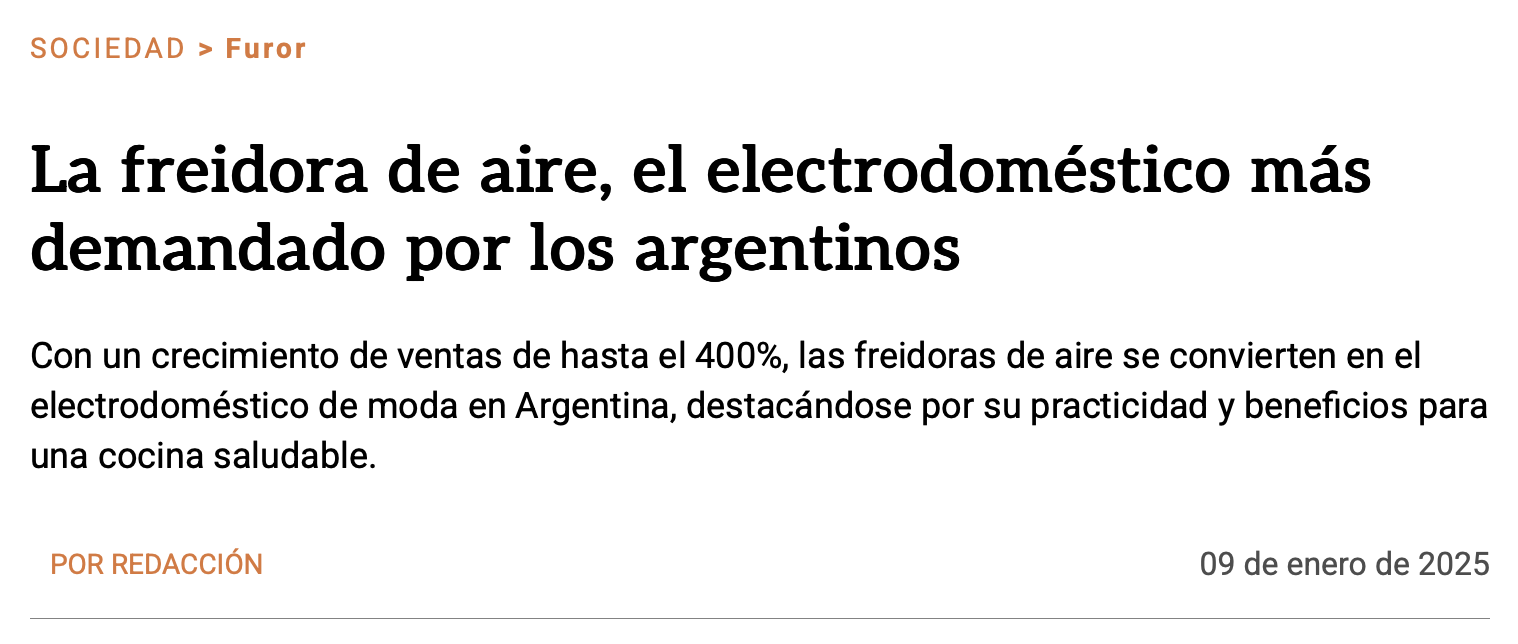
\includegraphics[scale=0.45]{Slides Principios de Economia/Figures/Magistral_04/M4.3.png}
    \end{center}
\end{frame}

\begin{frame}
\frametitle{Algunos ejemplos - Shocks externos}
    \begin{center}
    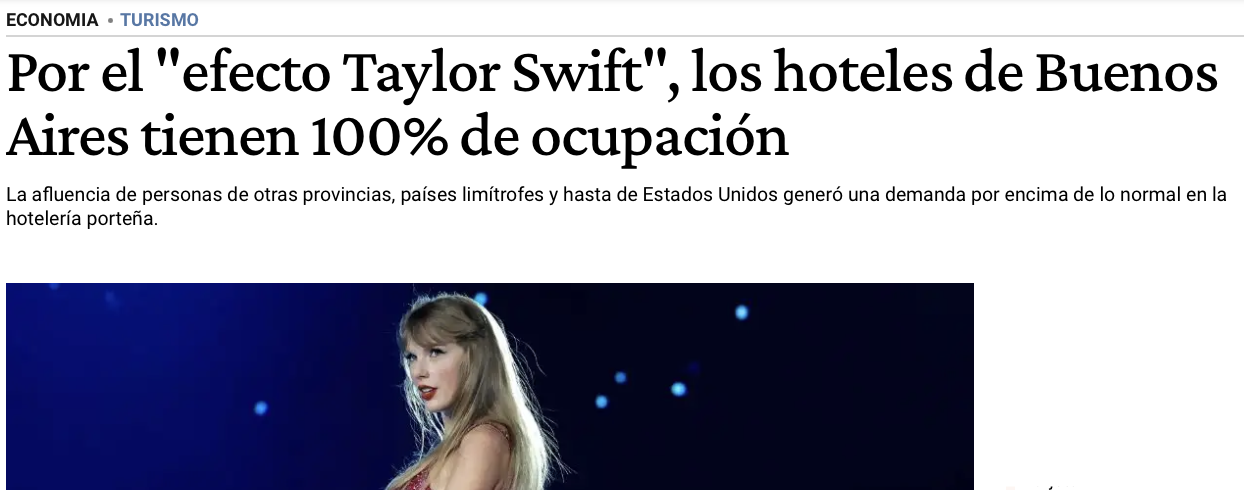
\includegraphics[scale=0.55]{Slides Principios de Economia/Figures/Magistral_04/M4.5.png}
    \end{center}
\end{frame}





\begin{frame}
\frametitle{¿Cómo se determina el ingreso?}
\begin{itemize}
    \item Hasta el momento, asumíamos que  conocíamos el ingreso sin preguntarnos como se obtenía. 
    \item Ahora vamos a utilizar las herramientas aprendidas para explicar cómo un individuo determina su ingreso laboral.
    \item A su vez, entender la decisión ocio-trabajo nos será de gran utilidad en la sección de macroeconomía. 
\end{itemize}
\end{frame}


\begin{frame}
\frametitle{Problema consumo - ocio}
\begin{itemize}
    \item Vamos a analizar cómo un individuo decide cuántas horas querrá trabajar por día y, eso definirá su ingreso.
    \item Enfrenta un trade-off entre dos bienes: las horas de tiempo libre (ocio) y el consumo en bienes.
    \item Hay un límite físico: la cantidad de horas por día que puede trabajar o disfrutar.
    \begin{equation}
     24 = H_{Ocio} + H_{Trabajo}.
    \end{equation}
    \item El costo de oportunidad del tiempo libre es el salario. 
    \item El consumo se define por la cantidad de horas de trabajo multiplicado por el salario:
    \begin{equation}
    Consumo = (24-H_{Ocio}) * Salario. 
    \end{equation}
\end{itemize}
\end{frame}


\begin{frame}
\frametitle{Gráficamente..}
Supongamos que el salario por hora es igual a \$10 \pause
    \begin{center}
    \begin{figure}[H]
    \renewcommand{\figurename}{Figure}
    \begin{center}
    \begin{tikzpicture}[scale=0.6]
    \draw[very thick,<->] (0,10) node[left]{Consumo}--(0,0)--(11,0) node[below]{Horas de ocio};
    \only<3->{
    \draw[fill] (7.5,0) circle [radius =0.12] node [below] {\footnotesize 24};
    }
    \only<4->{
    \draw[fill] (0,6.5) circle [radius =0.12] node [left] {\footnotesize \$240};
    }
    \only<5->{
    \draw[thin](0,6.5)--(7.5,0);
    \draw[thick, dashed,gray] (4.75,2.3)--(4.75,0);
    \draw[thick, dashed,gray] (4.75,2.3)--(0 ,2.3);
    \node[below] at (4.75,0){\footnotesize 19};
    \node[left] at (0,2.3){\footnotesize \$ 50};
    }

    \end{tikzpicture}
    \end{center}
    \label{fig:C6.17}
    \end{figure}
    \end{center}
\end{frame}

\begin{frame}
\frametitle{La TMT en el modelo ocio - consumo}
    \begin{center}
    \begin{figure}[H]
    \renewcommand{\figurename}{Figure}
    \begin{center}
    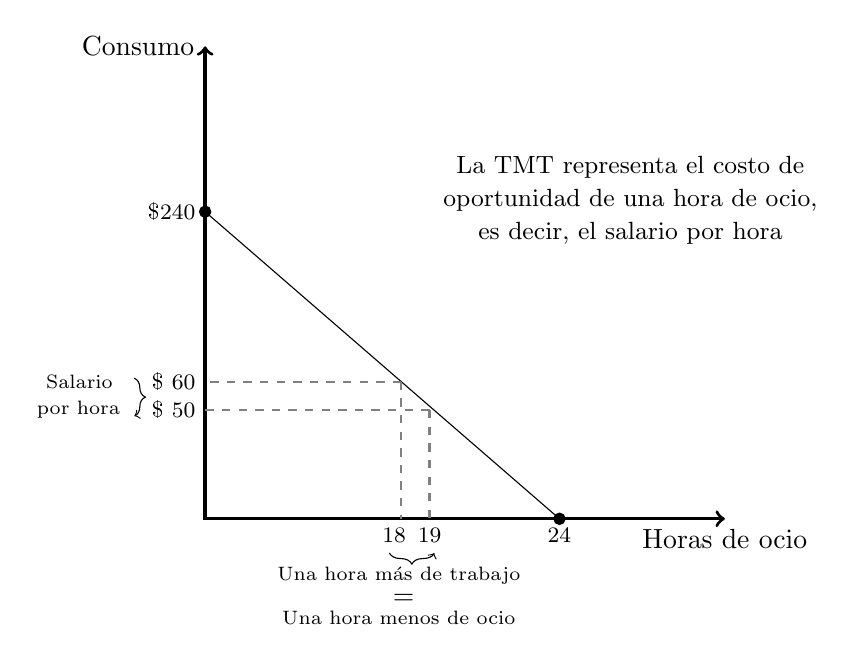
\begin{tikzpicture}[scale=0.6]
    \draw[very thick,<->] (0,10) node[left]{Consumo}--(0,0)--(11,0) node[below]{Horas de ocio};
    \draw[thin](0,6.5)--(7.5,0);
    \draw[thick, dashed,gray] (4.75,2.3)--(4.75,0);
    \draw[thick, dashed,gray] (4.75,2.3)--(0 ,2.3);
    \draw[thick, dashed,gray] (4.15,2.9)--(4.15,0);
    \draw[thick, dashed,gray] (4.15,2.9)--(0 ,2.9);
    \node[below] at (4.75,0){\footnotesize 19};
    \node[left] at (0,2.3){\footnotesize \$ 50};
    \node[below] at (4,0){\footnotesize 18};
    \node[left] at (0,2.9){\footnotesize \$ 60};
    \draw[fill] (0,6.5) circle [radius =0.12] node [left] {\footnotesize \$240};
    \draw [thin,->, decorate,decoration={brace,amplitude=4pt},xshift=0pt,yshift=5pt] (-1.5,2.8) -- (-1.5,2);
    \draw [thin,->,decorate,decoration={brace,amplitude=4pt, mirror},xshift=0pt,yshift=5pt](3.9,-0.9) -- (4.85,-0.9);
    \draw[fill] (7.5,0) circle [radius =0.12] node [below] {\footnotesize 24};
      \node[left] at (-1.75,2.9){\scriptsize Salario};   
        \node[left] at (-1.6,2.3){\scriptsize por hora};
          \node[] at (4.1,-1.2){\scriptsize Una hora más de trabajo}; 
        \node[] at (4.2,-1.7){=}; 
        \node[] at (4.1,-2.1){\scriptsize Una hora menos de ocio};
        \node[above] at (9,7) {\small La TMT representa el costo de};
        \node[above] at (9,6.3) {\small oportunidad de una hora de ocio,};
        \node[above] at (9,5.6) {\small es decir, el salario por hora};
    \end{tikzpicture}
    \end{center}
    \end{figure}
    \end{center}
\end{frame}

\begin{frame}
  \frametitle{La TMS en el modelo ocio - consumo} \vspace{3mm}
    La TMS representa la cantidad de consumo que el individuo está dispuesto a resignar por una hora más de tiempo libre, de manera tal que se mantenga constante su utilidad.
  \begin{center}
    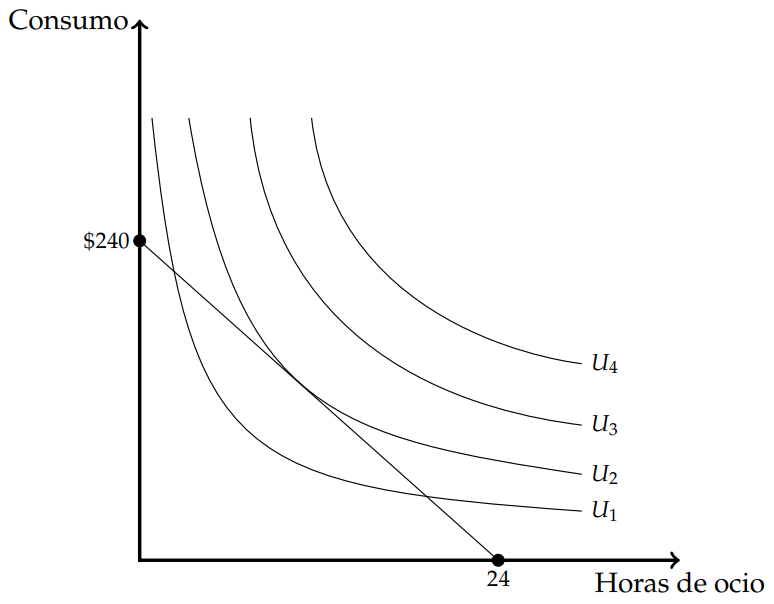
\includegraphics[scale=0.3]{Slides Principios de Economia/Figures/Magistral_04/C9.3.png}
  \end{center}
\end{frame}

\begin{frame}
\frametitle{El equilibrio}
    \begin{center}
    \begin{figure}[H]
    \renewcommand{\figurename}{Figure}
    \begin{center}
    \begin{tikzpicture}[scale=0.6]
    \draw[very thick,<->] (0,11) node[left]{Consumo}--(0,0)--(11,0) node[right]{Horas de ocio};
    \draw[thin] (1.75,9).. controls (2.15,4.35) and (7, 3) .. (9, 2.75) node [right]{\footnotesize $U_3$};
     \draw[thin] (0,8)--(9.75,0) ;
     \draw[thick,gray,dashed] (3.9,0)--(3.9,4.9)--(0,4.85);
    \draw[fill] (3.9,4.85) circle [radius =0.11] node [above] {\scriptsize A};
    % \draw[fill] (1.4,6.9) circle [radius =0.11] node [above] {\scriptsize B};      
    % \draw[fill] (2.2,6.2) circle [radius =0.11] node [above] {\scriptsize C};  
    % \node[below] at (1.4,0) {\footnotesize 5};
    % \node[below] at (2.2,0) {\footnotesize 6};
    \node[below] at (3.9,0) {\footnotesize 14};
    \node[below] at (9.75,0) {\footnotesize 24};
    \node[left] at (0,8) {\footnotesize \$ 240};
    \node[left] at (0,4.85) {\footnotesize \$ 100};
    % \node[left] at (0,6.2) {\footnotesize \$ 900};
    % \node[left] at (0,6.9) {\footnotesize \$ 950};
    \end{tikzpicture}
    \end{center}
    \end{figure}
    \end{center}

\end{frame}


\begin{frame}
\frametitle{¿Por qué G no es un equilibrio?}
\begin{center}
\begin{figure}[H]
\renewcommand{\figurename}{Figure}
\begin{center}
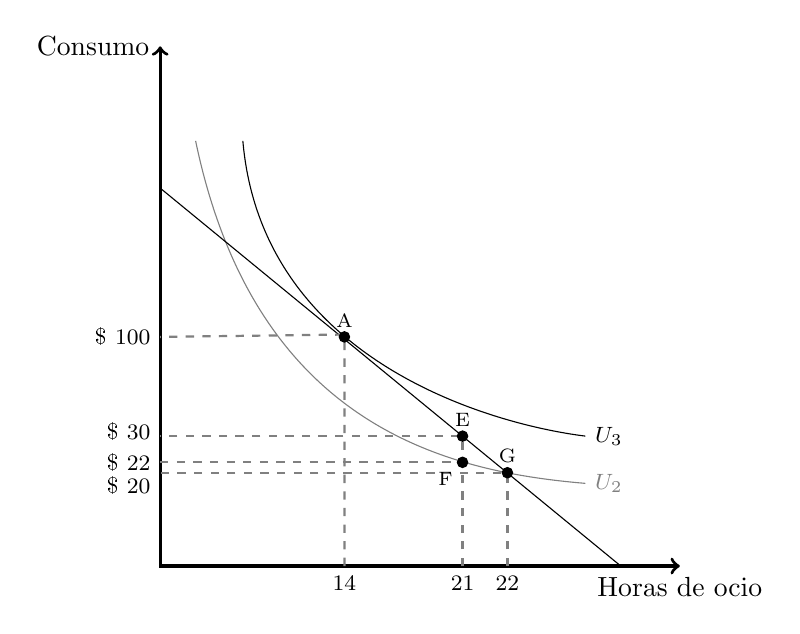
\begin{tikzpicture}[scale=0.6]
\draw[very thick,<->] (0,11) node[left]{Consumo}--(0,0)--(11,0) node[below]{Horas de ocio};
\draw[thin, gray] (0.75,9).. controls (2,3) and (6, 2) .. (9, 1.75) node [right]{\footnotesize $U_2$} ;
\draw[thin] (1.75,9).. controls (2.15,4.35) and (7, 3) .. (9, 2.75) node [right]{\footnotesize $U_3$};
 \draw[thin] (0,8)--(9.75,0) ;
 \draw[thick,gray,dashed] (3.9,0)--(3.9,4.9)--(0,4.85);
%  \draw[thick,gray,dashed] (1.4,0)--(1.4,6.9)--(0,6.9);
% \draw[thick,gray,dashed] (2.2,0)--(2.2,6.2)--(0,6.2); 
\draw[thick,gray,dashed] (6.4,0)--(6.4,2.75)--(0,2.75);
\draw[thick,gray,dashed] (7.35,0)--(7.35,1.975)--(0,1.975);
\draw[thick,gray,dashed] (0,2.195)--(6.4,2.195);
\draw[fill] (3.9,4.85) circle [radius =0.11] node [above] {\scriptsize A};
\draw[fill] (7.35,1.975) circle [radius =0.11] node [above] {\scriptsize G};
\draw[fill] (6.4,2.195) circle [radius =0.11] node [below left] {\scriptsize F};
\draw[fill] (6.4,2.75) circle [radius =0.11] node [above] {\scriptsize E};
% \draw[fill] (1.4,6.9) circle [radius =0.11] node [above] {\scriptsize B};      
% \draw[fill] (2.2,6.2) circle [radius =0.11] node [above] {\scriptsize C};  
% \node[below] at (1.4,0) {\footnotesize 5};
% \node[below] at (2.2,0) {\footnotesize 6};
\node[below] at (3.9,0) {\footnotesize 14};
\node[below] at (6.4,0) {\footnotesize 21};
\node[below] at (7.35,0) {\footnotesize 22};
\node[left] at (0,1.7) {\footnotesize \$ 20};
\node[left] at (0,2.195) {\footnotesize \$ 22};
\node[left] at (0,2.85) {\footnotesize \$ 30};
\node[left] at (0,4.85) {\footnotesize \$ 100};
% \node[left] at (0,6.2) {\footnotesize \$ 900};
% \node[left] at (0,6.9) {\footnotesize \$ 950};
\end{tikzpicture}
\end{center}
\end{figure}
\end{center}
\end{frame}


\begin{frame}
\frametitle{¿Por qué B no es un equilibrio?}
\begin{center}
\begin{figure}[H]
\renewcommand{\figurename}{Figure}
\begin{center}
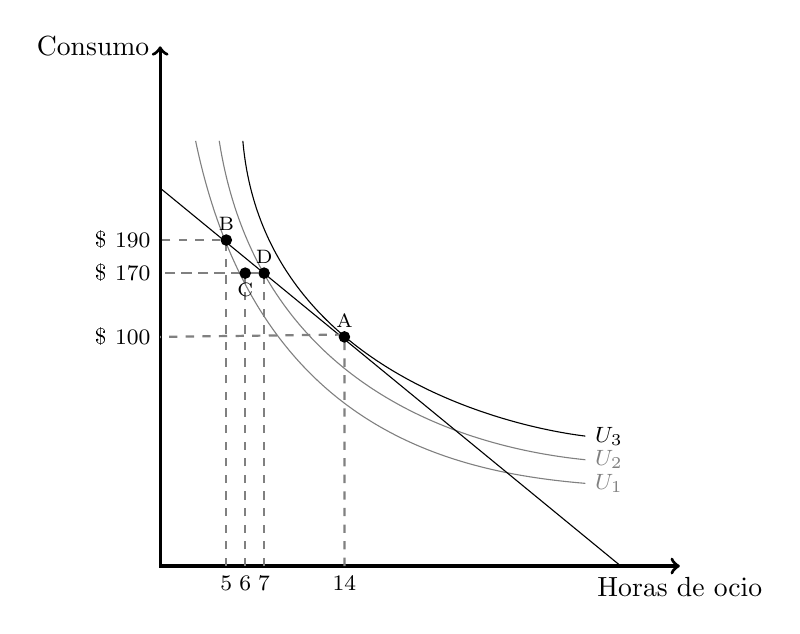
\begin{tikzpicture}[scale=0.6]
\draw[very thick,<->] (0,11) node[left]{Consumo}--(0,0)--(11,0) node[below]{Horas de ocio};
\draw[thin, gray] (0.75,9).. controls (2,3) and (6, 2) .. (9, 1.75) node [right]{\footnotesize $U_1$} ;
\draw[thin, gray] (1.25,9).. controls (2.07,3.75) and (6.5, 2.5) .. (9, 2.25) node [right]{\footnotesize $U_2$} ;
\draw[thin] (1.75,9).. controls (2.15,4.35) and (7, 3) .. (9, 2.75) node [right]{\footnotesize $U_3$};
 \draw[thin] (0,8)--(9.75,0) ;
 \draw[thick,gray,dashed] (3.9,0)--(3.9,4.9)--(0,4.85);
\draw[thick,gray,dashed] (1.4,0)--(1.4,6.9)--(0,6.9);
\draw[thick,gray,dashed] (1.8,0)--(1.8,6.2)--(0,6.2); 
\draw[thick,gray,dashed] (2.2,0)--(2.2,6.2)--(0,6.2); 
\draw[fill] (3.9,4.85) circle [radius =0.11] node [above] {\scriptsize A};
\draw[fill] (1.4,6.9) circle [radius =0.11] node [above] {\scriptsize B};      
\draw[fill] (1.8,6.2) circle [radius =0.11] node [below] {\scriptsize C};  
\draw[fill] (2.2,6.2) circle [radius =0.11] node [above] {\scriptsize D};  
\node[below] at (1.4,0) {\footnotesize 5};
\node[below] at (1.8,0) {\footnotesize 6};
\node[below] at (2.2,0) {\footnotesize 7};
\node[below] at (3.9,0) {\footnotesize 14};
\node[left] at (0,4.85) {\footnotesize \$ 100};
\node[left] at (0,6.2) {\footnotesize \$ 170};
\node[left] at (0,6.9) {\footnotesize \$ 190};
\end{tikzpicture}
\end{center}
\end{figure}
\end{center}
\end{frame}

\begin{frame}
  \frametitle{Un shock de ingreso extra}
  Supongamos que hay un shock de ingresos no relacionado al salario (por ejemplo, un regalo)
  \begin{center}
    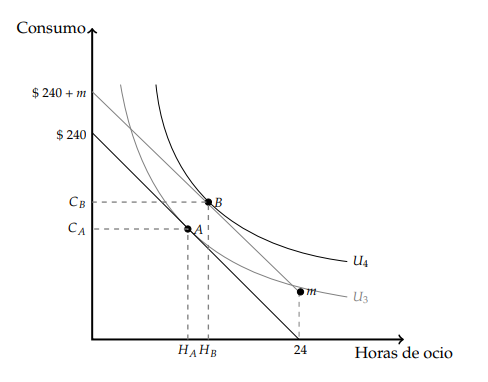
\includegraphics[scale=0.4]{Slides Principios de Economia/Figures/Magistral_04/C9.7.png}
  \end{center}
  En el nuevo equilibrio, el individuo aumenta tanto la cantidad de horas de ocio como su consumo.
\end{frame}

\begin{frame}
    \frametitle{Un aumento del salario}
    Si aumenta el salario, podemos hacer nuevamente la descomposición entre efecto ingreso y efecto sustitución. \vspace{2mm} \pause
  \begin{itemize}  
        \item El \textbf{efecto ingreso} está relacionado con el cambio en la decisión de ocio- trabajo como consecuencia de un cambio en el ingreso. 
        \begin{itemize}
        \item Con el aumento del salario, se puede mantener el nivel de consumo con menos horas de trabajo $\Rightarrow$ el individuo prefiere trabajar menos y tener más ocio. \vspace{2mm} \pause
        \end{itemize}
        \item El \textbf{efecto sustitución} está relacionado al aumento en el costo de oportunidad del ocio. 
        \begin{itemize}
        \item Cuando el salario aumenta, perder una hora de trabajo implica perder un salario más alto $\Rightarrow$ el individuo prefiere trabajar más y reducir su tiempo de ocio. \pause
        \end{itemize}
        \end{itemize}
    \begin{boxB}
        \centering El \textbf{efecto final} sobre la cantidad de horas de ocio-trabajo \textbf{va a depender de qué efecto predomina}
    \end{boxB}
\end{frame}

\begin{frame}
  \frametitle{Un aumento del salario}
  \begin{center}
    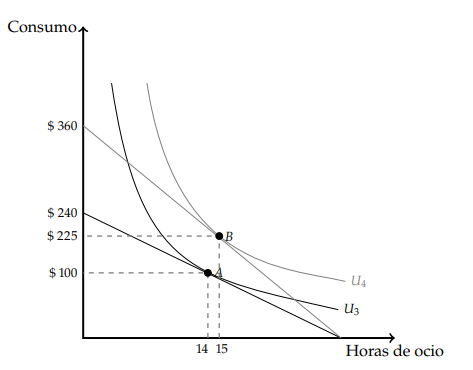
\includegraphics[scale=0.45]{Slides Principios de Economia/Figures/Magistral_04/C9.8.png}
  \end{center}
    En este caso, efecto ingreso $>$ efecto sustitución (aumentan el ocio)
\end{frame}

\begin{frame}
  \frametitle{Un aumento del salario II}
  \begin{center}
    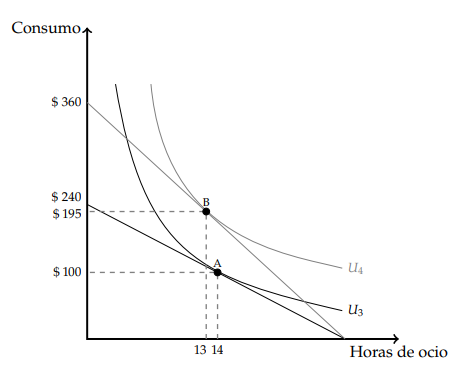
\includegraphics[scale=0.5]{Slides Principios de Economia/Figures/Magistral_04/C9.9.png}
  \end{center}
    En este caso, efecto ingreso $<$ efecto sustitución (disminuye el ocio)
\end{frame}

\begin{frame}
  \frametitle{Descomponiendo el efecto total}
  \begin{center}
    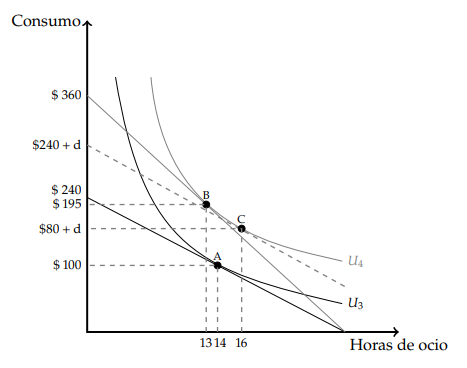
\includegraphics[scale=0.55]{Slides Principios de Economia/Figures/Magistral_04/C9.10.png}
  \end{center}
\end{frame}

\begin{frame}
  \frametitle{Descomponiendo el efecto total}
  \begin{center}
    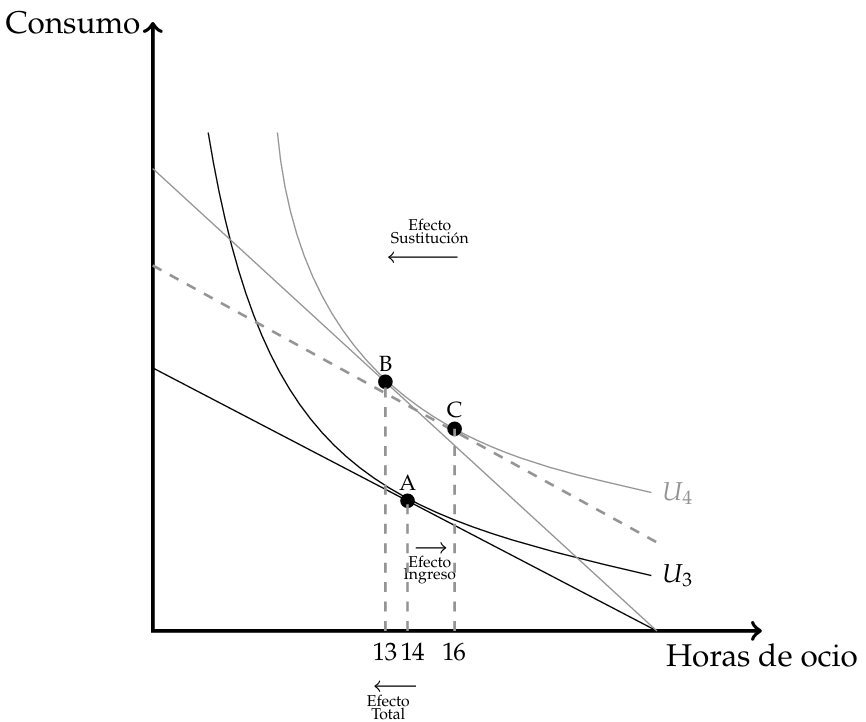
\includegraphics[scale=0.55]{Slides Principios de Economia/Figures/Magistral_04/C9.11.png}
  \end{center}
\end{frame}

\begin{frame}
  \frametitle{El largo plazo}
  \begin{itemize}
    \item En la práctica parece ser que hay una compensación exacta entre el efecto sustitución y el efecto ingreso.
    \item Eso quiere decir que los aumentos visualizados en el ingreso a lo largo de la historia no se tradujeron en una baja muy grande del tiempo trabajado.
    \item En el corto plazo, puede cambiar alguna decisión, pero no solemos pensar en el ocio como un bien normal (o sea que cuando aumenta el costo de oportunidad -salario- aumente mi consumo de ocio) ni como un bien inferior (cuando aumenta el salario - costo de oportunidad del ocio - disminuya el consumo de ocio).
  \end{itemize}
\end{frame}


\end{document}